% Options for packages loaded elsewhere
\PassOptionsToPackage{unicode}{hyperref}
\PassOptionsToPackage{hyphens}{url}
%
\documentclass[
]{article}
\usepackage{lmodern}
\usepackage{amssymb,amsmath}
\usepackage{ifxetex,ifluatex}
\ifnum 0\ifxetex 1\fi\ifluatex 1\fi=0 % if pdftex
  \usepackage[T1]{fontenc}
  \usepackage[utf8]{inputenc}
  \usepackage{textcomp} % provide euro and other symbols
\else % if luatex or xetex
  \usepackage{unicode-math}
  \defaultfontfeatures{Scale=MatchLowercase}
  \defaultfontfeatures[\rmfamily]{Ligatures=TeX,Scale=1}
\fi
% Use upquote if available, for straight quotes in verbatim environments
\IfFileExists{upquote.sty}{\usepackage{upquote}}{}
\IfFileExists{microtype.sty}{% use microtype if available
  \usepackage[]{microtype}
  \UseMicrotypeSet[protrusion]{basicmath} % disable protrusion for tt fonts
}{}
\makeatletter
\@ifundefined{KOMAClassName}{% if non-KOMA class
  \IfFileExists{parskip.sty}{%
    \usepackage{parskip}
  }{% else
    \setlength{\parindent}{0pt}
    \setlength{\parskip}{6pt plus 2pt minus 1pt}}
}{% if KOMA class
  \KOMAoptions{parskip=half}}
\makeatother
\usepackage{xcolor}
\IfFileExists{xurl.sty}{\usepackage{xurl}}{} % add URL line breaks if available
\IfFileExists{bookmark.sty}{\usepackage{bookmark}}{\usepackage{hyperref}}
\hypersetup{
  pdftitle={Prediction of hotel's Price in Vienna},
  pdfauthor={Maeva\_Braeckevelt},
  hidelinks,
  pdfcreator={LaTeX via pandoc}}
\urlstyle{same} % disable monospaced font for URLs
\usepackage[margin=1in]{geometry}
\usepackage{longtable,booktabs}
% Correct order of tables after \paragraph or \subparagraph
\usepackage{etoolbox}
\makeatletter
\patchcmd\longtable{\par}{\if@noskipsec\mbox{}\fi\par}{}{}
\makeatother
% Allow footnotes in longtable head/foot
\IfFileExists{footnotehyper.sty}{\usepackage{footnotehyper}}{\usepackage{footnote}}
\makesavenoteenv{longtable}
\usepackage{graphicx,grffile}
\makeatletter
\def\maxwidth{\ifdim\Gin@nat@width>\linewidth\linewidth\else\Gin@nat@width\fi}
\def\maxheight{\ifdim\Gin@nat@height>\textheight\textheight\else\Gin@nat@height\fi}
\makeatother
% Scale images if necessary, so that they will not overflow the page
% margins by default, and it is still possible to overwrite the defaults
% using explicit options in \includegraphics[width, height, ...]{}
\setkeys{Gin}{width=\maxwidth,height=\maxheight,keepaspectratio}
% Set default figure placement to htbp
\makeatletter
\def\fps@figure{htbp}
\makeatother
\setlength{\emergencystretch}{3em} % prevent overfull lines
\providecommand{\tightlist}{%
  \setlength{\itemsep}{0pt}\setlength{\parskip}{0pt}}
\setcounter{secnumdepth}{-\maxdimen} % remove section numbering
\usepackage{array}
\usepackage{caption}
\usepackage{graphicx}
\usepackage{siunitx}
\usepackage{ulem}
\usepackage{colortbl}
\usepackage{multirow}
\usepackage{hhline}
\usepackage{calc}
\usepackage{tabularx}
\usepackage{threeparttable}
\usepackage{wrapfig}
\usepackage{adjustbox}
\usepackage{hyperref}

\title{Prediction of hotel's Price in Vienna}
\author{Maeva\_Braeckevelt}
\date{12/02/2021}

\begin{document}
\maketitle

\hypertarget{summary}{%
\section{Summary}\label{summary}}

This analysis aimed at comparing best deals in hotels in Vienna found
with my models to the one we found during our analysis in chapter 10. I
used three different models: OLS, CART and Ramdom forest. After
comparing the RMSE and Rsquare, I chose the Random forest Model as my
best model. I run it again on my whole sample with my best parameters. I
predicted the price of my hotels and calculated my residuals. From my
fives best deals (lowest residuals), I had three in common with the
previous analysis from chapter 10.

\hypertarget{introduction}{%
\section{Introduction}\label{introduction}}

This analysis aimed at predicting the price of hotels in Vienna in order
to find the best deals.The data used was gathered in a csv files : The
hotels-vienna.csv. My predicted variable is the price in euro (y). My
sample the hotels in Vienna in the weekday of November 2017.

\hypertarget{data}{%
\section{Data}\label{data}}

\hypertarget{label-engineering}{%
\subsection{Label engineering}\label{label-engineering}}

My predicted variable is the price of hotel in Euro. I kept only the
price under 400 euro. The minimun price for a night is 27 euro and the
maximum 384 euro. The mean is 122.9 euro. I observed that the
distribution of the price is skewed with a right tail and some extreme
values. I did not transform my y variable to simplify my interpretation
of the residuals.

\begin{longtable}[]{@{}cccccc@{}}
\toprule
\begin{minipage}[b]{0.08\columnwidth}\centering
Min.\strut
\end{minipage} & \begin{minipage}[b]{0.12\columnwidth}\centering
1st Qu.\strut
\end{minipage} & \begin{minipage}[b]{0.10\columnwidth}\centering
Median\strut
\end{minipage} & \begin{minipage}[b]{0.09\columnwidth}\centering
Mean\strut
\end{minipage} & \begin{minipage}[b]{0.12\columnwidth}\centering
3rd Qu.\strut
\end{minipage} & \begin{minipage}[b]{0.08\columnwidth}\centering
Max.\strut
\end{minipage}\tabularnewline
\midrule
\endhead
\begin{minipage}[t]{0.08\columnwidth}\centering
27\strut
\end{minipage} & \begin{minipage}[t]{0.12\columnwidth}\centering
83\strut
\end{minipage} & \begin{minipage}[t]{0.10\columnwidth}\centering
109.5\strut
\end{minipage} & \begin{minipage}[t]{0.09\columnwidth}\centering
131.4\strut
\end{minipage} & \begin{minipage}[t]{0.12\columnwidth}\centering
146\strut
\end{minipage} & \begin{minipage}[t]{0.08\columnwidth}\centering
1012\strut
\end{minipage}\tabularnewline
\bottomrule
\end{longtable}

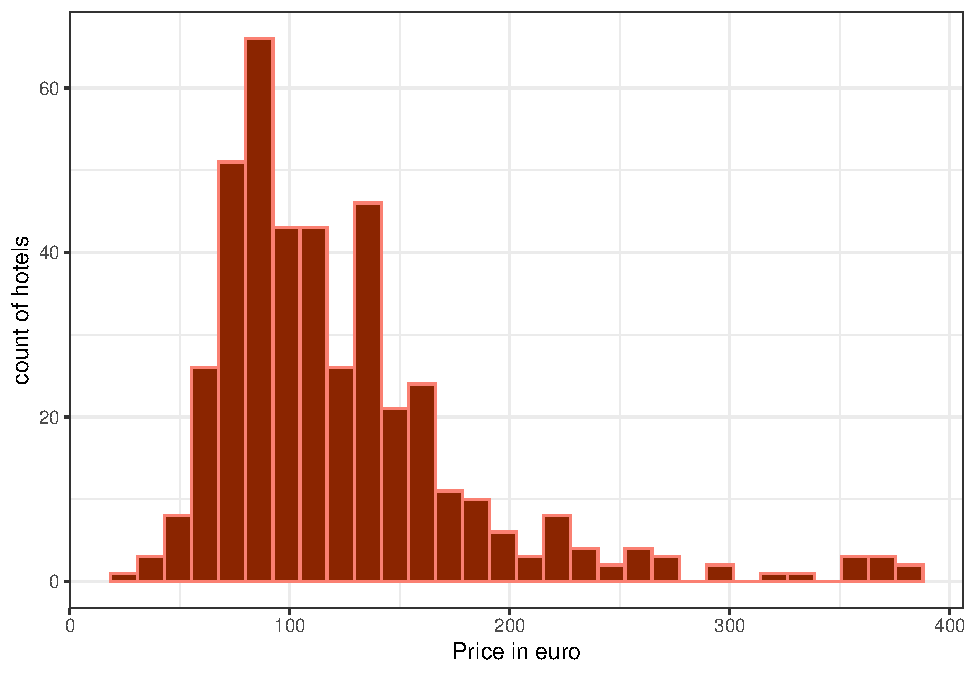
\includegraphics{Rmd_Maeva_Braeckevelt_prediction_price_vienna_files/figure-latex/unnamed-chunk-3-1.pdf}

\hypertarget{feature-engeneering}{%
\subsection{Feature Engeneering}\label{feature-engeneering}}

I decided to categorize my X variable in 4 categories :

\textbf{Location}

\begin{itemize}
\item
  Neigbhourhood : I factorized all the different neigbhourhood, and if a
  neigbhourhood appears less than 5 times in the sample, it is
  categorized as small\_neigbhourhood.
\item
  Distance : It is the distance from the city center, I only kept hotels
  that were maximum 5km away of the city center
\item
  Distance\_alter : It is the distance from the Donauturm.
\end{itemize}

\textbf{Rating}

\begin{itemize}
\item
  Stars : This variable shows the total of stars of the hotels
\item
  Rating : It's the user rating average, they were some missing values
  that I replace by 0, I did not flag them because, no other hotels had
  0 as rating and I did not want to add variable if it was not needed
\item
  Rating\_count : It is the number of user ratings, they were some
  missing values that I replace by 0, I did not flag them because, no
  other hotels had 0 rating and I did not want to add variable if it was
  not needed
\item
  Ratingta : It's the user rating average from the website Tripadvisor,
  they were some missing values that I replace by 0, I did not flag them
  because, no other hotels had 0 as rating and I did not want to add
  variable if it was not needed
\item
  Ratingta\_count : It is the number of user ratings in the tripadvisor
  website, they were some missing values that I replace by 0, I did not
  flag them because, no other hotels had 0 rating and I did not want to
  add variable if it was not needed
\end{itemize}

\textbf{Value}

\begin{itemize}
\item
  Scarce\_room : This variable was flagged, if room was noted as scarce
\item
  Offer : This variable was flagged, if there was an offer available
\item
  Offer\_cat : The offers for the roooms were categorized
\end{itemize}

\textbf{Interactions}

I choose my interactions with common knowledge :

\begin{itemize}
\item
  Distance with stars
\item
  Distance\_alter with stars
\item
  Distance with rating
\item
  Distance\_alter with rating
\end{itemize}

I decided to keep only hotels as a type of accommodation and only those
that were in the actual city of Vienna. My sample is composed by 246
observations.

\hypertarget{models}{%
\section{Models}\label{models}}

I chose my models by gradually add more categories at each model.

\begin{itemize}
\item
  \textbf{X1} : Location
\item
  \textbf{X2} : Location, \emph{rating}
\item
  \textbf{X3} : Location, rating, \emph{value}
\item
  \textbf{X4} : Location, rating, value, \emph{interactions}
\end{itemize}

\hypertarget{hold-out-set-and-cross-validation}{%
\subsection{Hold out set and cross
validation}\label{hold-out-set-and-cross-validation}}

I will not do an holdhout set because I only have 246 observations and
my goal is not to predict price for a live data but find the best deals
in my actual data. However, I will do a 5-fold cross-validation to
estimate models.

\hypertarget{models-1}{%
\subsection{Models}\label{models-1}}

I used three different kind of models : OLS, CART and Random forest. For
the OLS, I did a model with every predictors: X1,X2,X3 and X4. From the
table below, I observed the model 3 is the best model : it had the
lowest RMSE, the second best Rsquare, and the second lowest BIC. I chose
to use this model for the Cart and the Random Forest. After taking the
average of all the folds of the cross validation, I got the result of
the second table below. I observed that the Random forest had the lowest
RMSE and the Higher Rsquares of the three models. I will rerun the model
(with no cross validation) on all the sample, with the best parameters
that I found : 5 mtry and 5 minimum node'size.

\begin{longtable}[]{@{}ccccccc@{}}
\caption{OLS}\tabularnewline
\toprule
\begin{minipage}[b]{0.12\columnwidth}\centering
rmse\_test\strut
\end{minipage} & \begin{minipage}[b]{0.13\columnwidth}\centering
rmse\_train\strut
\end{minipage} & \begin{minipage}[b]{0.13\columnwidth}\centering
model\_name\strut
\end{minipage} & \begin{minipage}[b]{0.19\columnwidth}\centering
model\_pretty\_name\strut
\end{minipage} & \begin{minipage}[b]{0.08\columnwidth}\centering
nvars\strut
\end{minipage} & \begin{minipage}[b]{0.09\columnwidth}\centering
r2\strut
\end{minipage} & \begin{minipage}[b]{0.09\columnwidth}\centering
BIC\strut
\end{minipage}\tabularnewline
\midrule
\endfirsthead
\toprule
\begin{minipage}[b]{0.12\columnwidth}\centering
rmse\_test\strut
\end{minipage} & \begin{minipage}[b]{0.13\columnwidth}\centering
rmse\_train\strut
\end{minipage} & \begin{minipage}[b]{0.13\columnwidth}\centering
model\_name\strut
\end{minipage} & \begin{minipage}[b]{0.19\columnwidth}\centering
model\_pretty\_name\strut
\end{minipage} & \begin{minipage}[b]{0.08\columnwidth}\centering
nvars\strut
\end{minipage} & \begin{minipage}[b]{0.09\columnwidth}\centering
r2\strut
\end{minipage} & \begin{minipage}[b]{0.09\columnwidth}\centering
BIC\strut
\end{minipage}\tabularnewline
\midrule
\endhead
\begin{minipage}[t]{0.12\columnwidth}\centering
49.44\strut
\end{minipage} & \begin{minipage}[t]{0.13\columnwidth}\centering
44.75\strut
\end{minipage} & \begin{minipage}[t]{0.13\columnwidth}\centering
model1\strut
\end{minipage} & \begin{minipage}[t]{0.19\columnwidth}\centering
(1)\strut
\end{minipage} & \begin{minipage}[t]{0.08\columnwidth}\centering
17\strut
\end{minipage} & \begin{minipage}[t]{0.09\columnwidth}\centering
0.4067\strut
\end{minipage} & \begin{minipage}[t]{0.09\columnwidth}\centering
2678\strut
\end{minipage}\tabularnewline
\begin{minipage}[t]{0.12\columnwidth}\centering
42.31\strut
\end{minipage} & \begin{minipage}[t]{0.13\columnwidth}\centering
36.46\strut
\end{minipage} & \begin{minipage}[t]{0.13\columnwidth}\centering
model2\strut
\end{minipage} & \begin{minipage}[t]{0.19\columnwidth}\centering
(2)\strut
\end{minipage} & \begin{minipage}[t]{0.08\columnwidth}\centering
22\strut
\end{minipage} & \begin{minipage}[t]{0.09\columnwidth}\centering
0.6009\strut
\end{minipage} & \begin{minipage}[t]{0.09\columnwidth}\centering
2608\strut
\end{minipage}\tabularnewline
\begin{minipage}[t]{0.12\columnwidth}\centering
41.75\strut
\end{minipage} & \begin{minipage}[t]{0.13\columnwidth}\centering
35.46\strut
\end{minipage} & \begin{minipage}[t]{0.13\columnwidth}\centering
model3\strut
\end{minipage} & \begin{minipage}[t]{0.19\columnwidth}\centering
(3)\strut
\end{minipage} & \begin{minipage}[t]{0.08\columnwidth}\centering
26\strut
\end{minipage} & \begin{minipage}[t]{0.09\columnwidth}\centering
0.6216\strut
\end{minipage} & \begin{minipage}[t]{0.09\columnwidth}\centering
2617\strut
\end{minipage}\tabularnewline
\begin{minipage}[t]{0.12\columnwidth}\centering
43.99\strut
\end{minipage} & \begin{minipage}[t]{0.13\columnwidth}\centering
34.66\strut
\end{minipage} & \begin{minipage}[t]{0.13\columnwidth}\centering
model4\strut
\end{minipage} & \begin{minipage}[t]{0.19\columnwidth}\centering
(4)\strut
\end{minipage} & \begin{minipage}[t]{0.08\columnwidth}\centering
30\strut
\end{minipage} & \begin{minipage}[t]{0.09\columnwidth}\centering
0.6342\strut
\end{minipage} & \begin{minipage}[t]{0.09\columnwidth}\centering
2631\strut
\end{minipage}\tabularnewline
\bottomrule
\end{longtable}

\begin{longtable}[]{@{}ccccccc@{}}
\caption{Cart \& Random forest}\tabularnewline
\toprule
\begin{minipage}[b]{0.21\columnwidth}\centering
~\strut
\end{minipage} & \begin{minipage}[b]{0.09\columnwidth}\centering
Min.\strut
\end{minipage} & \begin{minipage}[b]{0.10\columnwidth}\centering
1st Qu.\strut
\end{minipage} & \begin{minipage}[b]{0.09\columnwidth}\centering
Median\strut
\end{minipage} & \begin{minipage}[b]{0.09\columnwidth}\centering
Mean\strut
\end{minipage} & \begin{minipage}[b]{0.10\columnwidth}\centering
3rd Qu.\strut
\end{minipage} & \begin{minipage}[b]{0.10\columnwidth}\centering
Max.\strut
\end{minipage}\tabularnewline
\midrule
\endfirsthead
\toprule
\begin{minipage}[b]{0.21\columnwidth}\centering
~\strut
\end{minipage} & \begin{minipage}[b]{0.09\columnwidth}\centering
Min.\strut
\end{minipage} & \begin{minipage}[b]{0.10\columnwidth}\centering
1st Qu.\strut
\end{minipage} & \begin{minipage}[b]{0.09\columnwidth}\centering
Median\strut
\end{minipage} & \begin{minipage}[b]{0.09\columnwidth}\centering
Mean\strut
\end{minipage} & \begin{minipage}[b]{0.10\columnwidth}\centering
3rd Qu.\strut
\end{minipage} & \begin{minipage}[b]{0.10\columnwidth}\centering
Max.\strut
\end{minipage}\tabularnewline
\midrule
\endhead
\begin{minipage}[t]{0.21\columnwidth}\centering
\textbf{CART\_RMSE}\strut
\end{minipage} & \begin{minipage}[t]{0.09\columnwidth}\centering
35.98\strut
\end{minipage} & \begin{minipage}[t]{0.10\columnwidth}\centering
38.2\strut
\end{minipage} & \begin{minipage}[t]{0.09\columnwidth}\centering
38.38\strut
\end{minipage} & \begin{minipage}[t]{0.09\columnwidth}\centering
40.92\strut
\end{minipage} & \begin{minipage}[t]{0.10\columnwidth}\centering
40.16\strut
\end{minipage} & \begin{minipage}[t]{0.10\columnwidth}\centering
51.87\strut
\end{minipage}\tabularnewline
\begin{minipage}[t]{0.21\columnwidth}\centering
\textbf{RF\_RMSE}\strut
\end{minipage} & \begin{minipage}[t]{0.09\columnwidth}\centering
29.09\strut
\end{minipage} & \begin{minipage}[t]{0.10\columnwidth}\centering
29.7\strut
\end{minipage} & \begin{minipage}[t]{0.09\columnwidth}\centering
29.95\strut
\end{minipage} & \begin{minipage}[t]{0.09\columnwidth}\centering
34.66\strut
\end{minipage} & \begin{minipage}[t]{0.10\columnwidth}\centering
34.27\strut
\end{minipage} & \begin{minipage}[t]{0.10\columnwidth}\centering
50.29\strut
\end{minipage}\tabularnewline
\begin{minipage}[t]{0.21\columnwidth}\centering
\textbf{CART\_Rsquared}\strut
\end{minipage} & \begin{minipage}[t]{0.09\columnwidth}\centering
0.3034\strut
\end{minipage} & \begin{minipage}[t]{0.10\columnwidth}\centering
0.4643\strut
\end{minipage} & \begin{minipage}[t]{0.09\columnwidth}\centering
0.5854\strut
\end{minipage} & \begin{minipage}[t]{0.09\columnwidth}\centering
0.5402\strut
\end{minipage} & \begin{minipage}[t]{0.10\columnwidth}\centering
0.5923\strut
\end{minipage} & \begin{minipage}[t]{0.10\columnwidth}\centering
0.7557\strut
\end{minipage}\tabularnewline
\begin{minipage}[t]{0.21\columnwidth}\centering
\textbf{RF\_Rsquared}\strut
\end{minipage} & \begin{minipage}[t]{0.09\columnwidth}\centering
0.3173\strut
\end{minipage} & \begin{minipage}[t]{0.10\columnwidth}\centering
0.631\strut
\end{minipage} & \begin{minipage}[t]{0.09\columnwidth}\centering
0.749\strut
\end{minipage} & \begin{minipage}[t]{0.09\columnwidth}\centering
0.6574\strut
\end{minipage} & \begin{minipage}[t]{0.10\columnwidth}\centering
0.7821\strut
\end{minipage} & \begin{minipage}[t]{0.10\columnwidth}\centering
0.8077\strut
\end{minipage}\tabularnewline
\bottomrule
\end{longtable}

\hypertarget{prediction}{%
\section{Prediction}\label{prediction}}

With my final model, I found my predicted value for my y variable : the
price of a room for one night. I could then calculate the residuals :
the difference between the real price and the predicted one. Find below,
the graph of those two values. I observed than my prediction is close to
the line, so my model is good.

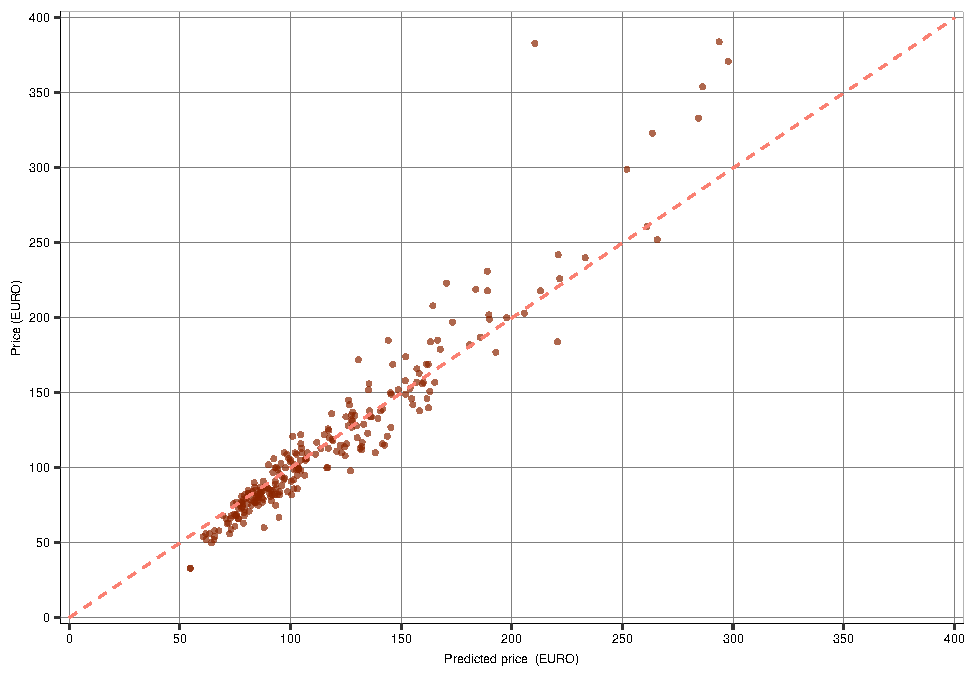
\includegraphics{Rmd_Maeva_Braeckevelt_prediction_price_vienna_files/figure-latex/unnamed-chunk-11-1.pdf}

\hypertarget{comparaison-of-the-5-best-deals}{%
\section{Comparaison of the 5 best
deals}\label{comparaison-of-the-5-best-deals}}

The five best deals of my sample, is the lowest residuals. Indeed, if
there is a big negative difference between the actual price and the
predicted price, it means that the hotels are cheaper than expected.
Find below the 5 best deals of my sample compare to the 5 best deals we
found in the chapter 10 with a different model.

\begin{longtable}[]{@{}cccccc@{}}
\caption{Best deals for hotels - Random forest}\tabularnewline
\toprule
\begin{minipage}[b]{0.13\columnwidth}\centering
hotel\_id\strut
\end{minipage} & \begin{minipage}[b]{0.09\columnwidth}\centering
price\strut
\end{minipage} & \begin{minipage}[b]{0.23\columnwidth}\centering
rf\_prediction\_res\strut
\end{minipage} & \begin{minipage}[b]{0.13\columnwidth}\centering
distance\strut
\end{minipage} & \begin{minipage}[b]{0.09\columnwidth}\centering
stars\strut
\end{minipage} & \begin{minipage}[b]{0.10\columnwidth}\centering
rating\strut
\end{minipage}\tabularnewline
\midrule
\endfirsthead
\toprule
\begin{minipage}[b]{0.13\columnwidth}\centering
hotel\_id\strut
\end{minipage} & \begin{minipage}[b]{0.09\columnwidth}\centering
price\strut
\end{minipage} & \begin{minipage}[b]{0.23\columnwidth}\centering
rf\_prediction\_res\strut
\end{minipage} & \begin{minipage}[b]{0.13\columnwidth}\centering
distance\strut
\end{minipage} & \begin{minipage}[b]{0.09\columnwidth}\centering
stars\strut
\end{minipage} & \begin{minipage}[b]{0.10\columnwidth}\centering
rating\strut
\end{minipage}\tabularnewline
\midrule
\endhead
\begin{minipage}[t]{0.13\columnwidth}\centering
22035\strut
\end{minipage} & \begin{minipage}[t]{0.09\columnwidth}\centering
184\strut
\end{minipage} & \begin{minipage}[t]{0.23\columnwidth}\centering
-36.64\strut
\end{minipage} & \begin{minipage}[t]{0.13\columnwidth}\centering
0.6\strut
\end{minipage} & \begin{minipage}[t]{0.09\columnwidth}\centering
5\strut
\end{minipage} & \begin{minipage}[t]{0.10\columnwidth}\centering
4.5\strut
\end{minipage}\tabularnewline
\begin{minipage}[t]{0.13\columnwidth}\centering
21984\strut
\end{minipage} & \begin{minipage}[t]{0.09\columnwidth}\centering
98\strut
\end{minipage} & \begin{minipage}[t]{0.23\columnwidth}\centering
-29.05\strut
\end{minipage} & \begin{minipage}[t]{0.13\columnwidth}\centering
0.5\strut
\end{minipage} & \begin{minipage}[t]{0.09\columnwidth}\centering
3\strut
\end{minipage} & \begin{minipage}[t]{0.10\columnwidth}\centering
3.7\strut
\end{minipage}\tabularnewline
\begin{minipage}[t]{0.13\columnwidth}\centering
22104\strut
\end{minipage} & \begin{minipage}[t]{0.09\columnwidth}\centering
110\strut
\end{minipage} & \begin{minipage}[t]{0.23\columnwidth}\centering
-28.28\strut
\end{minipage} & \begin{minipage}[t]{0.13\columnwidth}\centering
0.6\strut
\end{minipage} & \begin{minipage}[t]{0.09\columnwidth}\centering
4\strut
\end{minipage} & \begin{minipage}[t]{0.10\columnwidth}\centering
4.3\strut
\end{minipage}\tabularnewline
\begin{minipage}[t]{0.13\columnwidth}\centering
21912\strut
\end{minipage} & \begin{minipage}[t]{0.09\columnwidth}\centering
60\strut
\end{minipage} & \begin{minipage}[t]{0.23\columnwidth}\centering
-28.04\strut
\end{minipage} & \begin{minipage}[t]{0.13\columnwidth}\centering
1.1\strut
\end{minipage} & \begin{minipage}[t]{0.09\columnwidth}\centering
4\strut
\end{minipage} & \begin{minipage}[t]{0.10\columnwidth}\centering
4.1\strut
\end{minipage}\tabularnewline
\begin{minipage}[t]{0.13\columnwidth}\centering
22205\strut
\end{minipage} & \begin{minipage}[t]{0.09\columnwidth}\centering
67\strut
\end{minipage} & \begin{minipage}[t]{0.23\columnwidth}\centering
-27.79\strut
\end{minipage} & \begin{minipage}[t]{0.13\columnwidth}\centering
1.8\strut
\end{minipage} & \begin{minipage}[t]{0.09\columnwidth}\centering
3\strut
\end{minipage} & \begin{minipage}[t]{0.10\columnwidth}\centering
4\strut
\end{minipage}\tabularnewline
\bottomrule
\end{longtable}

\begin{longtable}[]{@{}cccccc@{}}
\caption{Best deals for hotels - Regression Chap10}\tabularnewline
\toprule
\begin{minipage}[b]{0.13\columnwidth}\centering
hotel\_id\strut
\end{minipage} & \begin{minipage}[b]{0.09\columnwidth}\centering
price\strut
\end{minipage} & \begin{minipage}[b]{0.23\columnwidth}\centering
rf\_prediction\_res\strut
\end{minipage} & \begin{minipage}[b]{0.13\columnwidth}\centering
distance\strut
\end{minipage} & \begin{minipage}[b]{0.09\columnwidth}\centering
stars\strut
\end{minipage} & \begin{minipage}[b]{0.10\columnwidth}\centering
rating\strut
\end{minipage}\tabularnewline
\midrule
\endfirsthead
\toprule
\begin{minipage}[b]{0.13\columnwidth}\centering
hotel\_id\strut
\end{minipage} & \begin{minipage}[b]{0.09\columnwidth}\centering
price\strut
\end{minipage} & \begin{minipage}[b]{0.23\columnwidth}\centering
rf\_prediction\_res\strut
\end{minipage} & \begin{minipage}[b]{0.13\columnwidth}\centering
distance\strut
\end{minipage} & \begin{minipage}[b]{0.09\columnwidth}\centering
stars\strut
\end{minipage} & \begin{minipage}[b]{0.10\columnwidth}\centering
rating\strut
\end{minipage}\tabularnewline
\midrule
\endhead
\begin{minipage}[t]{0.13\columnwidth}\centering
21912\strut
\end{minipage} & \begin{minipage}[t]{0.09\columnwidth}\centering
60\strut
\end{minipage} & \begin{minipage}[t]{0.23\columnwidth}\centering
-28.04\strut
\end{minipage} & \begin{minipage}[t]{0.13\columnwidth}\centering
1.1\strut
\end{minipage} & \begin{minipage}[t]{0.09\columnwidth}\centering
4\strut
\end{minipage} & \begin{minipage}[t]{0.10\columnwidth}\centering
4.1\strut
\end{minipage}\tabularnewline
\begin{minipage}[t]{0.13\columnwidth}\centering
21975\strut
\end{minipage} & \begin{minipage}[t]{0.09\columnwidth}\centering
115\strut
\end{minipage} & \begin{minipage}[t]{0.23\columnwidth}\centering
-27.46\strut
\end{minipage} & \begin{minipage}[t]{0.13\columnwidth}\centering
0.1\strut
\end{minipage} & \begin{minipage}[t]{0.09\columnwidth}\centering
4\strut
\end{minipage} & \begin{minipage}[t]{0.10\columnwidth}\centering
4.3\strut
\end{minipage}\tabularnewline
\begin{minipage}[t]{0.13\columnwidth}\centering
22080\strut
\end{minipage} & \begin{minipage}[t]{0.09\columnwidth}\centering
54\strut
\end{minipage} & \begin{minipage}[t]{0.23\columnwidth}\centering
-11.74\strut
\end{minipage} & \begin{minipage}[t]{0.13\columnwidth}\centering
1.1\strut
\end{minipage} & \begin{minipage}[t]{0.09\columnwidth}\centering
3\strut
\end{minipage} & \begin{minipage}[t]{0.10\columnwidth}\centering
3.2\strut
\end{minipage}\tabularnewline
\begin{minipage}[t]{0.13\columnwidth}\centering
22184\strut
\end{minipage} & \begin{minipage}[t]{0.09\columnwidth}\centering
75\strut
\end{minipage} & \begin{minipage}[t]{0.23\columnwidth}\centering
-18.32\strut
\end{minipage} & \begin{minipage}[t]{0.13\columnwidth}\centering
0.7\strut
\end{minipage} & \begin{minipage}[t]{0.09\columnwidth}\centering
3\strut
\end{minipage} & \begin{minipage}[t]{0.10\columnwidth}\centering
4.1\strut
\end{minipage}\tabularnewline
\begin{minipage}[t]{0.13\columnwidth}\centering
22344\strut
\end{minipage} & \begin{minipage}[t]{0.09\columnwidth}\centering
50\strut
\end{minipage} & \begin{minipage}[t]{0.23\columnwidth}\centering
-14.3\strut
\end{minipage} & \begin{minipage}[t]{0.13\columnwidth}\centering
3.9\strut
\end{minipage} & \begin{minipage}[t]{0.09\columnwidth}\centering
3\strut
\end{minipage} & \begin{minipage}[t]{0.10\columnwidth}\centering
3.9\strut
\end{minipage}\tabularnewline
\bottomrule
\end{longtable}

I observed that the hotels are totally different, it could be because,
in chapter 10, we kept only 3 and 4 stars hotel while in this sample I
kept all the star. So I filter to only 3 an 4 stars and then now I have
three hotels in common.

\begin{longtable}[]{@{}cccccc@{}}
\caption{Best deals for 3 and 4 stars hotels - Random
forest}\tabularnewline
\toprule
\begin{minipage}[b]{0.13\columnwidth}\centering
hotel\_id\strut
\end{minipage} & \begin{minipage}[b]{0.09\columnwidth}\centering
price\strut
\end{minipage} & \begin{minipage}[b]{0.23\columnwidth}\centering
rf\_prediction\_res\strut
\end{minipage} & \begin{minipage}[b]{0.13\columnwidth}\centering
distance\strut
\end{minipage} & \begin{minipage}[b]{0.09\columnwidth}\centering
stars\strut
\end{minipage} & \begin{minipage}[b]{0.10\columnwidth}\centering
rating\strut
\end{minipage}\tabularnewline
\midrule
\endfirsthead
\toprule
\begin{minipage}[b]{0.13\columnwidth}\centering
hotel\_id\strut
\end{minipage} & \begin{minipage}[b]{0.09\columnwidth}\centering
price\strut
\end{minipage} & \begin{minipage}[b]{0.23\columnwidth}\centering
rf\_prediction\_res\strut
\end{minipage} & \begin{minipage}[b]{0.13\columnwidth}\centering
distance\strut
\end{minipage} & \begin{minipage}[b]{0.09\columnwidth}\centering
stars\strut
\end{minipage} & \begin{minipage}[b]{0.10\columnwidth}\centering
rating\strut
\end{minipage}\tabularnewline
\midrule
\endhead
\begin{minipage}[t]{0.13\columnwidth}\centering
21984\strut
\end{minipage} & \begin{minipage}[t]{0.09\columnwidth}\centering
98\strut
\end{minipage} & \begin{minipage}[t]{0.23\columnwidth}\centering
-29.05\strut
\end{minipage} & \begin{minipage}[t]{0.13\columnwidth}\centering
0.5\strut
\end{minipage} & \begin{minipage}[t]{0.09\columnwidth}\centering
3\strut
\end{minipage} & \begin{minipage}[t]{0.10\columnwidth}\centering
3.7\strut
\end{minipage}\tabularnewline
\begin{minipage}[t]{0.13\columnwidth}\centering
22104\strut
\end{minipage} & \begin{minipage}[t]{0.09\columnwidth}\centering
110\strut
\end{minipage} & \begin{minipage}[t]{0.23\columnwidth}\centering
-28.28\strut
\end{minipage} & \begin{minipage}[t]{0.13\columnwidth}\centering
0.6\strut
\end{minipage} & \begin{minipage}[t]{0.09\columnwidth}\centering
4\strut
\end{minipage} & \begin{minipage}[t]{0.10\columnwidth}\centering
4.3\strut
\end{minipage}\tabularnewline
\begin{minipage}[t]{0.13\columnwidth}\centering
21912\strut
\end{minipage} & \begin{minipage}[t]{0.09\columnwidth}\centering
60\strut
\end{minipage} & \begin{minipage}[t]{0.23\columnwidth}\centering
-28.04\strut
\end{minipage} & \begin{minipage}[t]{0.13\columnwidth}\centering
1.1\strut
\end{minipage} & \begin{minipage}[t]{0.09\columnwidth}\centering
4\strut
\end{minipage} & \begin{minipage}[t]{0.10\columnwidth}\centering
4.1\strut
\end{minipage}\tabularnewline
\begin{minipage}[t]{0.13\columnwidth}\centering
22205\strut
\end{minipage} & \begin{minipage}[t]{0.09\columnwidth}\centering
67\strut
\end{minipage} & \begin{minipage}[t]{0.23\columnwidth}\centering
-27.79\strut
\end{minipage} & \begin{minipage}[t]{0.13\columnwidth}\centering
1.8\strut
\end{minipage} & \begin{minipage}[t]{0.09\columnwidth}\centering
3\strut
\end{minipage} & \begin{minipage}[t]{0.10\columnwidth}\centering
4\strut
\end{minipage}\tabularnewline
\begin{minipage}[t]{0.13\columnwidth}\centering
21975\strut
\end{minipage} & \begin{minipage}[t]{0.09\columnwidth}\centering
115\strut
\end{minipage} & \begin{minipage}[t]{0.23\columnwidth}\centering
-27.46\strut
\end{minipage} & \begin{minipage}[t]{0.13\columnwidth}\centering
0.1\strut
\end{minipage} & \begin{minipage}[t]{0.09\columnwidth}\centering
4\strut
\end{minipage} & \begin{minipage}[t]{0.10\columnwidth}\centering
4.3\strut
\end{minipage}\tabularnewline
\bottomrule
\end{longtable}

\hypertarget{conclusion}{%
\section{Conclusion}\label{conclusion}}

This analysis aimed at comparing best deals in hotels in Vienna found
with my models to the one we found during our analysis in chapter 10. I
used three different models: OLS, CART and Ramdom forest. After
comparing the RMSE and Rsquare, I chose the Random forest Model as my
best model. I run it again on my whole sample with my best parameters. I
predicted the price of my hotels and calculated my residuals. From my
fives best deals (lowest residuals), I had three in common with the
previous analysis from chapter 10.

\end{document}
